% CSC411: Assignment 1
% Due: Friday, February 3, 2017
% Zi Mo Su (1001575048)
%
%%%%%%%%%%%%%%%%%%%%%%%%%%%%%%%%%%%%%%%%%
% Programming/Coding Assignment
% LaTeX Template
%
% This template has been downloaded from:
% http://www.latextemplates.com
%
% Original author:
% Ted Pavlic (http://www.tedpavlic.com)
%
% Note:
% The \lipsum[#] commands throughout this template generate dummy text
% to fill the template out. These commands should all be removed when 
% writing assignment content.
%
% This template uses a Perl script as an example snippet of code, most other
% languages are also usable. Configure them in the "CODE INCLUSION 
% CONFIGURATION" section.
%
%%%%%%%%%%%%%%%%%%%%%%%%%%%%%%%%%%%%%%%%%

%----------------------------------------------------------------------------------------
%	PACKAGES AND OTHER DOCUMENT CONFIGURATIONS
%----------------------------------------------------------------------------------------

\documentclass{article}

\usepackage{fancyhdr} % Required for custom headers
\usepackage{lastpage} % Required to determine the last page for the footer
\usepackage{extramarks} % Required for headers and footers
\usepackage[usenames,dvipsnames]{color} % Required for custom colors
\usepackage{graphicx} % Required to insert images
\usepackage{subcaption}
\usepackage{listings} % Required for insertion of code
\usepackage{courier} % Required for the courier font
\usepackage{lipsum} % Used for inserting dummy 'Lorem ipsum' text into the template
\usepackage{bm}
\usepackage{pgfplots} % Used for plots
\pgfplotsset{width=10cm,compat=1.9}
\usepackage{amsmath} % Used for matrices

% Margins
\topmargin=-0.45in
\evensidemargin=0in
\oddsidemargin=0in
\textwidth=6.5in
\textheight=9.0in
\headsep=0.25in

\linespread{1.1} % Line spacing

% Set up the header and footer
\pagestyle{fancy}
\lhead{\hmwkAuthorName} % Top left header
\chead{\hmwkClass\ (\hmwkClassTime): \hmwkTitle} % Top center head
%\rhead{\firstxmark} % Top right header
\lfoot{\lastxmark} % Bottom left footer
\cfoot{} % Bottom center footer
\rfoot{Page\ \thepage\ of\ \protect\pageref{LastPage}} % Bottom right footer
\renewcommand\headrulewidth{0.4pt} % Size of the header rule
\renewcommand\footrulewidth{0.4pt} % Size of the footer rule

\setlength\parindent{0pt} % Removes all indentation from paragraphs

%----------------------------------------------------------------------------------------
%	CODE INCLUSION CONFIGURATION
%----------------------------------------------------------------------------------------

\definecolor{MyDarkGreen}{rgb}{0.0,0.4,0.0} % This is the color used for comments
\lstloadlanguages{Perl} % Load Perl syntax for listings, for a list of other languages supported see: ftp://ftp.tex.ac.uk/tex-archive/macros/latex/contrib/listings/listings.pdf
\lstset{language=Perl, % Use Perl in this example
        frame=single, % Single frame around code
        basicstyle=\small\ttfamily, % Use small true type font
        keywordstyle=[1]\color{Blue}\bf, % Perl functions bold and blue
        keywordstyle=[2]\color{Purple}, % Perl function arguments purple
        keywordstyle=[3]\color{Blue}\underbar, % Custom functions underlined and blue
        identifierstyle=, % Nothing special about identifiers                                         
        commentstyle=\usefont{T1}{pcr}{m}{sl}\color{MyDarkGreen}\small, % Comments small dark green courier font
        stringstyle=\color{Purple}, % Strings are purple
        showstringspaces=false, % Don't put marks in string spaces
        tabsize=5, % 5 spaces per tab
        %
        % Put standard Perl functions not included in the default language here
        morekeywords={rand},
        %
        % Put Perl function parameters here
        morekeywords=[2]{on, off, interp},
        %
        % Put user defined functions here
        morekeywords=[3]{test},
       	%
        morecomment=[l][\color{Blue}]{...}, % Line continuation (...) like blue comment
        numbers=left, % Line numbers on left
        firstnumber=1, % Line numbers start with line 1
        numberstyle=\tiny\color{Blue}, % Line numbers are blue and small
        stepnumber=5 % Line numbers go in steps of 5
}

% Creates a new command to include a perl script, the first parameter is the filename of the script (without .pl), the second parameter is the caption
\newcommand{\perlscript}[2]{
\begin{itemize}
\item[]\lstinputlisting[caption=#2,label=#1]{#1.pl}
\end{itemize}
}

%----------------------------------------------------------------------------------------
%	DOCUMENT STRUCTURE COMMANDS
%	Skip this unless you know what you're doing
%----------------------------------------------------------------------------------------

% Header and footer for when a page split occurs within a problem environment
\newcommand{\enterProblemHeader}[1]{
%\nobreak\extramarks{#1}{#1 continued on next page\ldots}\nobreak
%\nobreak\extramarks{#1 (continued)}{#1 continued on next page\ldots}\nobreak
}

% Header and footer for when a page split occurs between problem environments
\newcommand{\exitProblemHeader}[1]{
%\nobreak\extramarks{#1 (continued)}{#1 continued on next page\ldots}\nobreak
%\nobreak\extramarks{#1}{}\nobreak
}

\setcounter{secnumdepth}{0} % Removes default section numbers
\newcounter{homeworkProblemCounter} % Creates a counter to keep track of the number of problems
\setcounter{homeworkProblemCounter}{0}

\newcommand{\homeworkProblemName}{}
\newenvironment{homeworkProblem}[1][Part \arabic{homeworkProblemCounter}]{ % Makes a new environment called homeworkProblem which takes 1 argument (custom name) but the default is "Part #"
\stepcounter{homeworkProblemCounter} % Increase counter for number of problems
\renewcommand{\homeworkProblemName}{#1} % Assign \homeworkProblemName the name of the problem
\section{\homeworkProblemName} % Make a section in the document with the custom problem count
\enterProblemHeader{\homeworkProblemName} % Header and footer within the environment
}{
\exitProblemHeader{\homeworkProblemName} % Header and footer after the environment
}

\newcommand{\problemAnswer}[1]{ % Defines the problem answer command with the content as the only argument
\noindent\framebox[\columnwidth][c]{\begin{minipage}{0.98\columnwidth}#1\end{minipage}} % Makes the box around the problem answer and puts the content inside
}

\newcommand{\homeworkSectionName}{}
\newenvironment{homeworkSection}[1]{ % New environment for sections within homework problems, takes 1 argument - the name of the section
\renewcommand{\homeworkSectionName}{#1} % Assign \homeworkSectionName to the name of the section from the environment argument
\subsection{\homeworkSectionName} % Make a subsection with the custom name of the subsection
\enterProblemHeader{\homeworkProblemName\ [\homeworkSectionName]} % Header and footer within the environment
}{
\enterProblemHeader{\homeworkProblemName} % Header and footer after the environment
}

%----------------------------------------------------------------------------------------
%	NAME AND CLASS SECTION
%----------------------------------------------------------------------------------------

\newcommand{\hmwkTitle}{Assignment\ 1} % Assignment title
\newcommand{\hmwkDueDate}{Friday,\ February\ 3,\ 2017} % Due date
\newcommand{\hmwkClass}{CSC411} % Course/class
\newcommand{\hmwkClassTime}{L2501} % Class/lecture time
\newcommand{\hmwkAuthorName}{Zi Mo Su (1001575048)} % Your name

%----------------------------------------------------------------------------------------
%	TITLE PAGE
%----------------------------------------------------------------------------------------

\title{
\vspace{2in}
\textmd{\textbf{\hmwkClass:\ \hmwkTitle}}\\
\normalsize\vspace{0.1in}\small{Due\ on\ \hmwkDueDate}\\
\vspace{0.1in}
\vspace{3in}
}

\author{\textbf{\hmwkAuthorName}}
%\date{} % Insert date here if you want it to appear below your name

%----------------------------------------------------------------------------------------

\begin{document}

\maketitle
\clearpage
%----------------------------------------------------------------------------------------
%	PART 1
%----------------------------------------------------------------------------------------

% To have just one problem per page, simply put a \clearpage after each problem

\begin{homeworkProblem}

\noindent \textit{Dataset description.}

The uncropped dataset consists of $1,940$ images of varying sizes. It is composed of six actors and six actresses, each with a varying number of images. For our purposes, we use 120 images of each actor/actress and we have split the actors/actresses into two groups, \texttt{act} and \texttt{act\_test}. Figure~\ref{fig:uncropped} shows examples of the raw data.

\begin{figure*}[h!]
    \centering
    \begin{subfigure}{.2\textwidth}
        \centering
        \includegraphics[height=2.4cm]{baldwin000.jpg}
    \end{subfigure}%
    \begin{subfigure}{.2\textwidth}
        \centering
        \includegraphics[height=2.4cm]{baldwin001.jpg}
    \end{subfigure}%
    \begin{subfigure}{.2\textwidth}
        \centering
        \includegraphics[height=2.4cm]{baldwin002.jpg}
    \end{subfigure}%
    \begin{subfigure}{.2\textwidth}
        \centering
        \includegraphics[height=2.4cm]{baldwin003.jpg}
    \end{subfigure}%
    \begin{subfigure}{.2\textwidth}
        \centering
        \includegraphics[height=2.4cm]{baldwin004.jpg}
    \end{subfigure}%
    \caption{Examples of the raw images (photos of Alec Baldwin).}
    \label{fig:uncropped}
\end{figure*}

The cropped dataset consists of $1,940$ grayscale $32\times 32$-pixel images. Each image is cropped such that the person's face dictates the boundary of the image, as shown in Figure~\ref{fig:cropped}.
\\

\begin{figure*}[h!]
    \centering
    \begin{subfigure}{.2\textwidth}
        \centering
        \includegraphics[height=2.4cm]{crop_baldwin000.jpg}
    \end{subfigure}%
    \begin{subfigure}{.2\textwidth}
        \centering
        \includegraphics[height=2.4cm]{crop_baldwin001.jpg}
    \end{subfigure}%
    \begin{subfigure}{.2\textwidth}
        \centering
        \includegraphics[height=2.4cm]{crop_baldwin002.jpg}
    \end{subfigure}%
    \begin{subfigure}{.2\textwidth}
        \centering
        \includegraphics[height=2.4cm]{crop_baldwin003.jpg}
    \end{subfigure}%
    \begin{subfigure}{.2\textwidth}
        \centering
        \includegraphics[height=2.4cm]{crop_baldwin004.jpg}
    \end{subfigure}%
    \caption{Examples of the cropped images (photos of Alec Baldwin).}
    \label{fig:cropped}
\end{figure*}

The alignment of the images in Figure~\ref{fig:cropped} is shown in Figure~\ref{fig:overlay}, where the transparency of each of the five images has been set to $90\%$ and they have been superimposed. We observe that the overlaid images align fairly accurately at the eyes, nose, mouth, and eyebrows; all of which are desired features of accentuation for facial recognition.

\begin{figure*}[h!]
    \centering
    \includegraphics[width=0.25\linewidth]{overlay.png}
    \caption{Superimposed images from Figure~\ref{fig:cropped}.}
    \label{fig:overlay}
\end{figure*}

The raw data comes in the form of a text file, the quality of which is sub-par; numerous images are corrupted and thus must be disposed of and some images are not of the actor/actress but have been removed and replaced with a filler by the source. The data itself is easily parse-able, however, making the preprocessing fairly simple.

\end{homeworkProblem}
\clearpage
%----------------------------------------------------------------------------------------
%	PART 2
%----------------------------------------------------------------------------------------

\begin{homeworkProblem}
\noindent \textit{Partitioning the dataset.}

The dataset, after preprocessing in Part 1, is stored in a dictionary. This dictionary contains key-value pairs of the form:\\

\texttt{\{baldwin000:2D array\}}\\

The key is the name of the file without its extension, and the value is the 2D numpy array representing the processed image.\\

This main dataset is taken and partitioned into a training set with 100 images per actor/actress, and a validation set and test set with 10 images each per actor/actress. The form of these sets is the same as the above dictionary for the master set. The \texttt{partition()} function is used to partition the set. It takes in the list of actors (e.g., \texttt{act}), the master set, and the sizes for the training, validation and test sets, which are by default 100, 10, and 10 respectively. Since the data is retrieved from a dictionary, the order is uncertain; as such, the data is partitioned according to the filename (e.g., \texttt{baldwin000}), specifically the number in the filename (e.g, \texttt{000}). The first 10 entries are parted to the validation set, the next 10 to the test set and the next 100 to the training set.

\newpage

The \texttt{partition()} function is shown below:\\

\lstinputlisting[language=Python, firstline=139, lastline=177, breaklines=True]{faces.py}

\end{homeworkProblem}
\clearpage
%----------------------------------------------------------------------------------------
%	PART 3
%----------------------------------------------------------------------------------------

\begin{homeworkProblem}
\noindent \textit{Building a classifier for two actors.}

A classifier for images of Bill Hader and Steve Carell is implemented in this part. The cost function minimized is:

$$J(\bm{\theta}) = \frac{1}{2m}\sum_{i=1}^{m}({y^{(i)}-\bm{x^{(i)}\theta^T}})^2$$

where $m$ is the number of images that are in the training set, $y^{(i)}$ is $-1$ if the $i^{th}$ image is of Bill Hader and $1$ if the image is of Steve Carell, $\bm{x^{(i)}}$ is a $1\times1025$ vector where the first element is $1$ and the next $1024$ are the pixels of the $32\times32$ image read left to right and top to bottom, and $\bm{\theta}$ is a $1\times1025$ vector with elements $\theta_0...\theta_{1024}$, which are the unknown parameters to be optimized over.
\\

The gradient descent algorithm was applied to the training set (size $100$) with $\epsilon=1\times10^{-6}$, $\alpha=1\times10^{-7}$. It took $3,369$ iterations and yielded the following results:

\begin{enumerate}
    \item[i.]Cost of the \textit{training set}: $J(\bm{\theta})=0.042$
    \item[ii.]Cost of the \textit{validation set}: $J(\bm{\theta})=0.42$
    \item[iii.]Performance of the \textit{training set}: $100.0\%$ accurate
    \item[iv.]Performance of the \textit{validation set}: $95.0\%$ accurate
\end{enumerate}

To make the gradient descent algorithm work, the parameter $\alpha$ had to be adjusted. When $\alpha$ was too large the system would diverge to infinity. When $\alpha$ was too small the system converged too quickly to a local minimum and thus resulted in poor performance. The $\alpha$ value was tuned by multiples of $10$ starting at $1\times10^{-4}$ to $1\times10^{-10}$, and it was found that $1\times10^{-7}$ yielded effective performance. It is important also to note that a smaller $\alpha$ may yield better performance but will result in longer runtime and overfitting.\\

Other parameters adjusted for gradient descent included $\epsilon$ and the number of max iterations. If $\epsilon$ is chosen very small, then it is likely the max iteration will be hit. Alternatively, a larger $\epsilon$ may result in completion of gradient descent before the max iteration is hit. $\epsilon$ was chosen to be $1\times10^{-6}$. Larger values were tested but resulted in poor performance, since the number of iterations was not enough. Smaller values resulted in extremely long runtimes between five and 10 minutes. The maximum number of iterations was set to $100,000$, however it is never reached in the reported results. 

\newpage
The following is the function used to compute the output of the classifier. If the computed hypothesis function, $\bm{x\theta^T}$, is less than zero, the image is classified as Bill Hader, otherwise it is classified as Steve Carell.
\\

\lstinputlisting[language=Python, firstline=289, lastline=322, breaklines=True]{faces.py}

\end{homeworkProblem}
\clearpage

%----------------------------------------------------------------------------------------
%	PART 4
%----------------------------------------------------------------------------------------

\begin{homeworkProblem}
\noindent \textit{Visualizing optimized $\theta$ parameters.}

The hypothesis function:

$$h_\theta(\bm{x})=\theta_0+\theta_1x_1+...+\theta_{1024}x_{1024}$$

is used to compute the approximation of the classification value. The $\theta$ parameters that correspond to a minimum for the cost function, generated through gradient descent, can be visualized as a $32\times32$ image, excluding $\theta_0$.\\

Two training sets are used to optimize the \bm{$\theta$} vector. One with 100 images of each actor and the other with two images of each actor. The results of the visualized \bm{$\theta$} vectors are shown in Figure~\ref{fig:part4}

\begin{figure*}[h!]
    \centering
    \begin{subfigure}{.4\textwidth}
      \centering
      \includegraphics[width=0.8\linewidth]{part4_1.jpg}
      \caption{The \bm{$\theta$} vector generated from a training set consisting of 100 pictures of each actor (Bill Hader and Steve Carell), visualized as an image.}
      \label{fig:part4_1}
    \end{subfigure}%
    \hspace{.02\textwidth}
    \begin{subfigure}{.4\textwidth}
      \centering
      \includegraphics[width=0.8\linewidth]{part4_2.jpg}
      \caption{The \bm{$\theta$} vector generated from a training set consisting of two pictures of each actor (Bill Hader and Steve Carell), visualized as an image.}
      \label{fig:part4_2}
    \end{subfigure}%
    \caption{}
    \label{fig:part4}
\end{figure*}

\end{homeworkProblem}
\clearpage

%----------------------------------------------------------------------------------------
%	PART 5
%----------------------------------------------------------------------------------------
\begin{homeworkProblem}
\noindent \textit{Demonstration of overfitting on gender classifiers.}

The gender classifiers used to classify actors/actresses as male or female were created by assigning $y=-1$ for actors and $y=1$ for actresses. Training sets varying in size by multiples of 10 images per actor/actress were used, starting at 10 images per actor/actress and ending at 100. The training set contains six different actors, three male and three female. The parameter $\alpha=1\times10^{-7}$ and the validation set were both held constant throughout the trials. The performance results of the validation set and training set are plotted against the training set size in Figure~\ref{fig:plot}.\\

\begin{figure*}[h!]
    \centering
    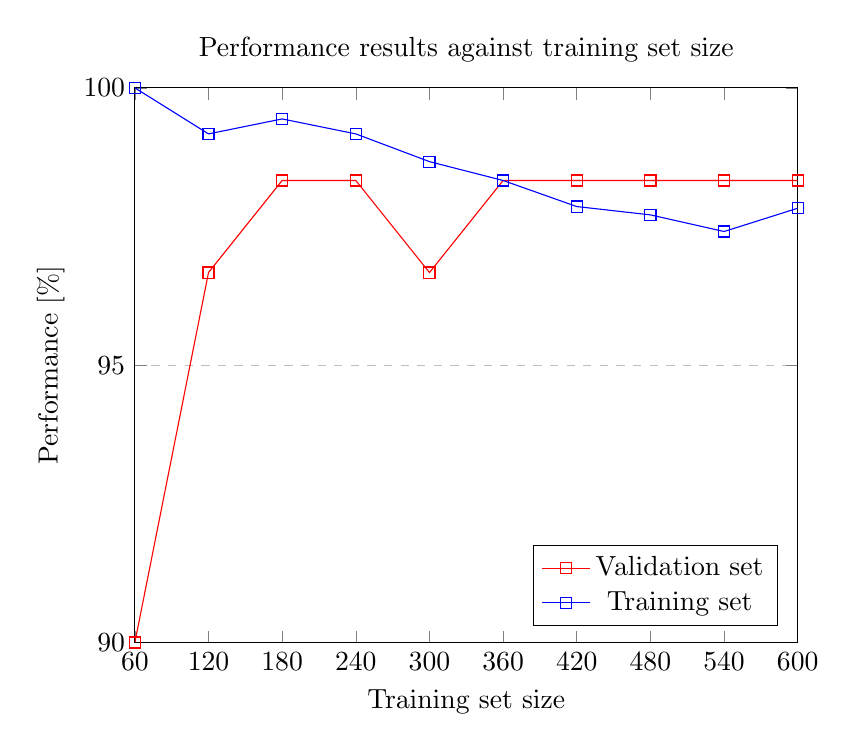
\begin{tikzpicture}
    \begin{axis}[
        title={Performance results against training set size},
        xlabel={Training set size},
        ylabel={Performance [\%]},
        xmin=60, xmax=600,
        ymin=90, ymax=100,
        xtick={60,120,180,240,300,360,420,480,540,600},
        ytick={90,95,100},
        legend pos=south east,
        ymajorgrids=true,
        grid style=dashed,
    ]
    
    \addplot[
        color=red,
        mark=square,
        ]
        coordinates {
        (60,90)(120,96.67)(180,98.33)(240,98.33)(300,96.67)(360,98.33)(420,98.33)(480,98.33)(540,98.33)(600,98.33)
        };
        
    \addplot[
        color=blue,
        mark=square,
        ]
        coordinates {
        (60,100)(120,99.17)(180,99.44)(240,99.17)(300,98.67)(360,98.33)(420,97.86)(480,97.71)(540,97.41)(600,97.83)
        };
        \legend{Validation set, Training set}
        
    \end{axis}
    \end{tikzpicture}
    \caption{}
    \label{fig:plot}
\end{figure*}

We observe the consistent decrease in performance of the training set. At a small training set size, it is easy to fit the training data accurately, hence the $100.0\%$ performance on the training set when the size is 60. As the size increases, the data becomes harder to fit, and thus poorer performance results arise. On the other hand, the validation set fits the data the worst at the beginning because of overfitting. The data is overfitting the training set; it captures patterns that are unique to the training set. As such, since these patterns are not exhibited in the validation set at times, the performance is lowered. In general, we observe the validation set performance remains stable after the first couple training set sizes. A larger training set results in poorer performance on the training data because the fit becomes more generalized.\\

Testing the classifier on the set of actors/actresses that are not in the training data (i.e., \texttt{act\_test}), yields an accuracy of $88.0\%$. This performance accuracy is quite good; as such it is fair to say that there is a significant enough difference between males and females for classification purposes. It would be interesting to observe the effects of added images of females with short hair and males with long hair.

\end{homeworkProblem}
\clearpage

%----------------------------------------------------------------------------------------
%	PART 6
%----------------------------------------------------------------------------------------
\begin{homeworkProblem}
\noindent \textit{Classification with multiple labels.}

\begin{enumerate}
    \item[a)]The cost function is:
    
    $$J(\bm{\Theta})=\sum_{i=1}^m\sum_{j=1}^k(\bm{\Theta}^T\bm{x^{(i)}}-\bm{y^{(i)}})_j^2$$
    
    For a single image, $\bm{\Theta}^T\bm{x^{(i)}}-\bm{y^{(i)}}$ is:
    \[
    \begin{bmatrix}
        \theta_{01} & \theta_{11} & \dots  & \theta_{(n-1)1} \\
        \theta_{02} & \theta_{12} & \dots  & \theta_{(n-1)2} \\
        \vdots & \vdots & \ddots & \vdots \\
        \theta_{0k} & \theta_{1k} & \dots  & \theta_{(n-1)k}
    \end{bmatrix}
    \begin{bmatrix}
        1 \\
        x_{1}^{(i)} \\
        \vdots \\
        x_{n-1}^{(i)}
    \end{bmatrix}
    -
    \begin{bmatrix}
        y_{1}^{(i)} \\
        y_{2}^{(i)} \\
        \vdots \\
        y_{k}^{(i)}
    \end{bmatrix}
    \]
    
    The expansion of which is:
    
    $$(\bm{\Theta}^T\bm{x^{(i)}}-\bm{y^{(i)}})_j=\theta_{0j}+\theta_{1j}x_1^{(i)}+...+\theta_{(n-1)j}x_{n-1}^{(i)}-y_{j}^{(i)}$$
    
    The partial derivative of the cost function with respect to $\theta_{pq}$ is thus:
    
    $$\frac{\partial J(\bm{\Theta})}{\partial\theta_{pq}}=2\sum_{i=1}^m\sum_{j=1}^k(\bm{\Theta}^T\bm{x^{(i)}}-\bm{y^{(i)}})_jx_p^{(i)}$$\\
    
    \item[b)]The following are definitions for $\bm{\Theta}$, $\bm{X}$, and $\bm{Y}$:
    
    $$\bm{\Theta}^T=
    \begin{bmatrix}
        \theta_{01} & \theta_{11} & \dots  & \theta_{(n-1)1} \\
        \theta_{02} & \theta_{12} & \dots  & \theta_{(n-1)2} \\
        \vdots & \vdots & \ddots & \vdots \\
        \theta_{0k} & \theta_{1k} & \dots  & \theta_{(n-1)k}
    \end{bmatrix}
    \in\Re^{k\times n}
    $$
    
    $$\bm{X}=
    \begin{bmatrix}
        1 & 1 & \dots  & 1 \\
        x_{1}^{(1)} & x_{1}^{(2)} & \dots  & x_{1}^{(m)} \\
        \vdots & \vdots & \ddots & \vdots \\
        x_{n-1}^{(1)} & x_{n-1}^{(2)} & \dots  & x_{n-1}^{(m)}
    \end{bmatrix}
    \in\Re^{n\times m}
    $$
    
    $$
    \bm{Y}=
    \begin{bmatrix}
        y_{0}^{(1)} & y_{0}^{(2)} & \dots  & y_{0}^{(m)} \\
        y_{1}^{(1)} & y_{1}^{(2)} & \dots  & y_{1}^{(m)} \\
        \vdots & \vdots & \ddots & \vdots \\
        y_{k}^{(1)} & y_{k}^{(2)} & \dots  & y_{k}^{(m)}
    \end{bmatrix}
    \in\Re^{k\times m}
    $$
    
    where $k$ is the number of labels ($6$), $m$ is the number of training images, and $n$ is one more than the number of pixels per image ($1025$).\\
    
    \newpage
    
    We can compute $(\bm{\Theta}^T\bm{X}-\bm{Y})^T$:
    
    $$(\bm{\Theta}^T\bm{X}-\bm{Y})^T=
    \begin{bmatrix}
        \bm{\Theta}^T\bm{x^{(1)}}-\bm{y^{(1)}} \\
        \bm{\Theta}^T\bm{x^{(2)}}-\bm{y^{(2)}} \\
        \vdots \\
        \bm{\Theta}^T\bm{x^{(m)}}-\bm{y^{(m)}}
    \end{bmatrix}
    $$
    
    where $\bm{x^{(i)}}$ and $\bm{y^{(i)}}$ are the $i^{th}$ columns of $\bm{X}$ and $\bm{Y}$, respectively.\\
    
    Multiplying $\bm{X}$ by this result yields:
    
    $$\bm{X}(\bm{\Theta}^T\bm{X}-\bm{Y})^T=
    \begin{bmatrix}
        \bm{x^{(1)}} & \bm{x^{(2)}} & \dots & \bm{x^{(m)}}
    \end{bmatrix}
    \begin{bmatrix}
        \bm{\Theta}^T\bm{x^{(1)}}-\bm{y^{(1)}} \\
        \bm{\Theta}^T\bm{x^{(2)}}-\bm{y^{(2)}} \\
        \vdots \\
        \bm{\Theta}^T\bm{x^{(m)}}-\bm{y^{(m)}}
    \end{bmatrix}
    $$
    
    This expands to:
    
    $$\bm{X}(\bm{\Theta}^T\bm{X}-\bm{Y})^T=
        \bm{x^{(1)}}(\bm{\Theta}^T\bm{x^{(1)}}-\bm{y^{(1)}}) + \bm{x^{(2)}}(\bm{\Theta}^T\bm{x^{(2)}}-\bm{y^{(2)}}) + ... + \bm{x^{(m)}}(\bm{\Theta}^T\bm{x^{(m)}}-\bm{y^{(m)}})
    $$
    
    Each element in this matrix is equal to the partial derivative found in part a) (without the coefficient 2). As such,
    
    $$\frac{\partial J(\bm{\Theta})}{\partial\bm{\Theta}}=2\bm{X}(\bm{\Theta}^T\bm{X}-\bm{Y})^T$$\\
    
    \item[c)]The cost function is implemented as follows in \texttt{f\_v()}:\\
    
    \lstinputlisting[language=Python, firstline=429, lastline=442, breaklines=True]{faces.py}
    
    \newpage
    
    The vectorized gradient is implemented as follows in \texttt{df\_v()}:\\
    
    \lstinputlisting[language=Python, firstline=444, lastline=455, breaklines=True]{faces.py}
    
    In this implementation, the coefficient of the cost function, $\frac{1}{2m}$, where $m$ is the number of images in the training set, has been included. This allows for efficient computation times and increased performance.\\
    
    \item[d)]The finite difference gradient is computed using the following code. At each $\theta_{ij}$, the partial derivative is calculated and placed in the gradient. The finite difference computation is shown below:\\
    
    \lstinputlisting[language=Python, firstline=457, lastline=478, breaklines=True]{faces.py}
    
    To identify the similarity between the analytically computed gradient and the numerically computed one through the finite difference method, we take the norm of the difference between the two. This is plotted against varying step sizes used in the finite difference computation, as shown in Figure~\ref{fig:finite_diff}.
    
    \newpage
    \begin{figure*}[h!]
    \centering
    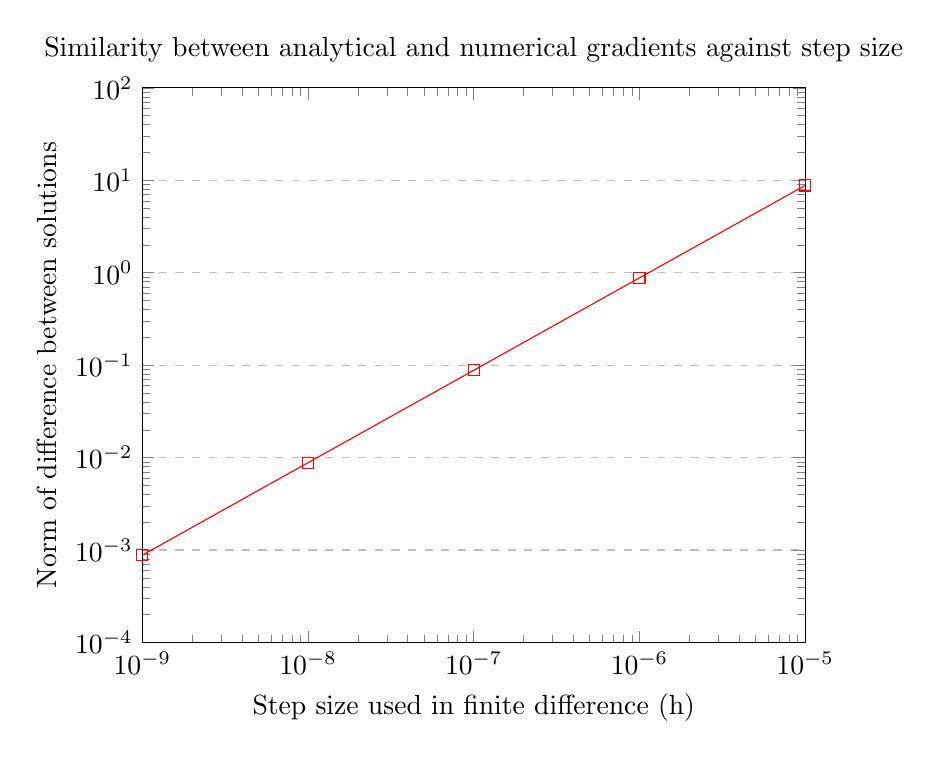
\begin{tikzpicture}
    \begin{axis}[
        title={Similarity between analytical and numerical
        gradients against step size},
        xlabel={Step size used in finite difference (h)},
        ylabel={Norm of difference between solutions},
        xmode=log,
        ymode=log,
        xmin=0.000000001, xmax=0.00001,
        ymin=0.0001, ymax=100,
        legend pos=north west,
        ymajorgrids=true,
        grid style=dashed,
    ]
    
    \addplot[
        color=red,
        mark=square,
        ]
        coordinates {
        (0.000000001,0.00088)(0.00000001,0.0088)(0.0000001,0.088)(0.000001,0.88)(0.00001,8.8)
        };
        
    \end{axis}
    \end{tikzpicture}
    \caption{}
    \label{fig:finite_diff}
\end{figure*}
    
    We see that as the step size used for the numerical computation of the gradient decreases, the difference between the analytical and numerical solutions decreases as well.
    
\end{enumerate}

\end{homeworkProblem}
\clearpage

%----------------------------------------------------------------------------------------
%	PART 7
%----------------------------------------------------------------------------------------
\begin{homeworkProblem}
\noindent \textit{Performance of facial recognition classifier.}

Using the set of actors/actresses in \texttt{act}, with 100 images of each actor/actress, training was executed with gradient descent. The performance of the classifier is shown in Figure~\ref{fig:fr_plot}.

\begin{figure*}[h!]
    \centering
    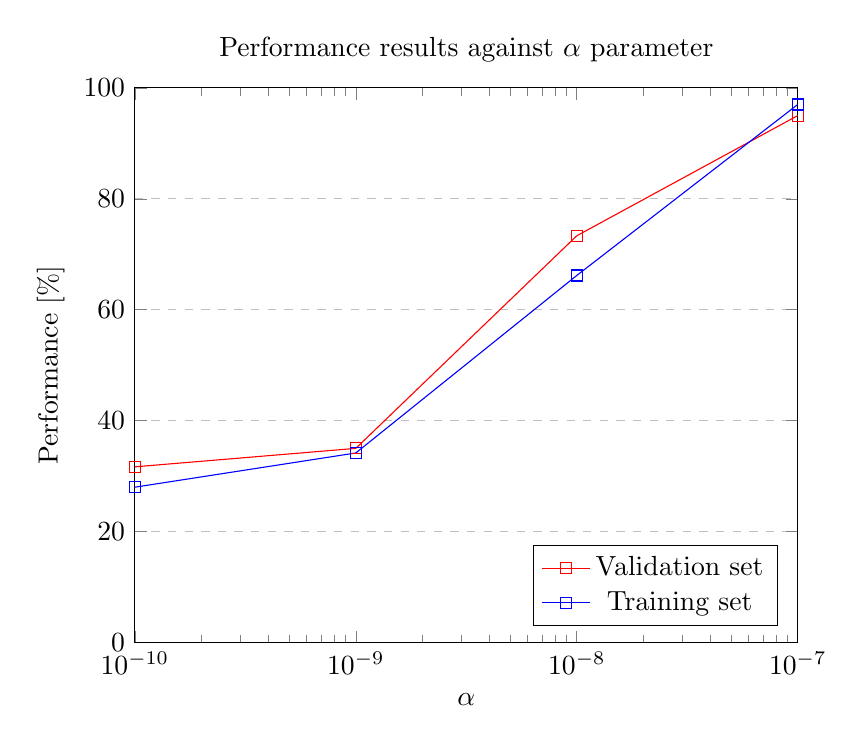
\begin{tikzpicture}
    \begin{axis}[
        title={Performance results against $\alpha$ parameter},
        xlabel={$\alpha$},
        ylabel={Performance [\%]},
        xmode=log,
        xmin=0.0000000001, xmax=0.0000001,
        ymin=0, ymax=100,
        xtick={0.0000000001, 0.000000001, 0.00000001, 0.0000001},
        ytick={0,20,40,60,80,100},
        legend pos=south east,
        ymajorgrids=true,
        grid style=dashed,
    ]
    
    \addplot[
        color=red,
        mark=square,
        ]
        coordinates {
        (0.0000000001,31.67)(0.000000001,35)(0.00000001,73.33)(0.0000001,95)
        };
        
    \addplot[
        color=blue,
        mark=square,
        ]
        coordinates {
        (0.0000000001,28)(0.000000001,34.17)(0.00000001,66.17)(0.0000001,97)
        };
        \legend{Validation set, Training set}
        
    \end{axis}
    \end{tikzpicture}
    \caption{}
    \label{fig:fr_plot}
\end{figure*}

We observe the classifier performs better as $\alpha$ increases. This is expected as the number of iterations also increases. A small $\alpha$ gets gradient descent to converge to a local minimum, resulting in a large cost. As the $\alpha$ value is increased, these local minima are surmounted and the convergence to a lower cost results in better performance. We note when $\alpha=1\times10^{-7}$, the performance of the training set is better than that of the validation set for the first time. This may be indicative of overfitting.

\end{homeworkProblem}
\clearpage

%----------------------------------------------------------------------------------------
%	PART 8
%----------------------------------------------------------------------------------------
\begin{homeworkProblem}
\noindent \textit{Visualizing optimized $\theta$ parameters with multiple classifications.}

Figure~\ref{fig:part8_1} shows the images of the theta parameters (extracted as in part 4). The actor/actress associated with the image is labeled. This result is observed when running with $\alpha=4\times10^{-9}$, which yields a performance of $50.0\%$ on the training set and $56.7\%$ on the validation set. Figure~\ref{fig:part8_2} and Figure~\ref{fig:part8_3} show the results for larger $\alpha$ values. Notice the decrease in fluency of the actors'/actresses' faces as a result of a better fitting and overfitting. The performance increases as expected since there are more iterations, reaching over $95.0\%$ performance on both sets at $\alpha=1\times10^{-7}$.

\begin{figure*}[h!]
    \centering
    \captionsetup{justification=centering,margin=2.2cm}
    \begin{subfigure}{.22\textwidth}
        \centering
        \includegraphics[width=.85\linewidth]{part8_1.jpg}
        \caption{Fran Drescher}
    \end{subfigure}%
    \begin{subfigure}{.22\textwidth}
        \centering
        \includegraphics[width=.85\linewidth]{part8_2.jpg}
        \caption{America Ferrera}
    \end{subfigure}%
    \begin{subfigure}{.22\textwidth}
        \centering
        \includegraphics[width=.85\linewidth]{part8_3.jpg}
        \caption{Kristin Chenoweth}
    \end{subfigure}%
    
    \begin{subfigure}{.22\textwidth}
        \centering
        \includegraphics[width=.85\linewidth]{part8_4.jpg}
        \caption{Alec Baldwin}
    \end{subfigure}%
    \begin{subfigure}{.22\textwidth}
        \centering
        \includegraphics[width=.85\linewidth]{part8_5.jpg}
        \caption{Bill Hader}
    \end{subfigure}%
    \begin{subfigure}{.22\textwidth}
        \centering
        \includegraphics[width=.85\linewidth]{part8_6.jpg}
        \caption{Steve Carell}
    \end{subfigure}%
    \caption{Visualizations of the $\theta$s using $\alpha=4\times10^{-9}$ with performance of $50.0\%$ (test) and $56.7\%$ (validation). The cost is 0.41 ending on iteration 43.}
    \label{fig:part8_1}
\end{figure*}

\begin{figure*}[h!]
    \centering
    \captionsetup{justification=centering,margin=2.2cm}
    \begin{subfigure}{.22\textwidth}
        \centering
        \includegraphics[width=.85\linewidth]{part8_1a.jpg}
        \caption{Fran Drescher}
    \end{subfigure}%
    \begin{subfigure}{.22\textwidth}
        \centering
        \includegraphics[width=.85\linewidth]{part8_2a.jpg}
        \caption{America Ferrera}
    \end{subfigure}%
    \begin{subfigure}{.22\textwidth}
        \centering
        \includegraphics[width=.85\linewidth]{part8_3a.jpg}
        \caption{Kristin Chenoweth}
    \end{subfigure}%
    
    \begin{subfigure}{.22\textwidth}
        \centering
        \includegraphics[width=.85\linewidth]{part8_4a.jpg}
        \caption{Alec Baldwin}
    \end{subfigure}%
    \begin{subfigure}{.22\textwidth}
        \centering
        \includegraphics[width=.85\linewidth]{part8_5a.jpg}
        \caption{Bill Hader}
    \end{subfigure}%
    \begin{subfigure}{.22\textwidth}
        \centering
        \includegraphics[width=.85\linewidth]{part8_6a.jpg}
        \caption{Steve Carell}
    \end{subfigure}%
    \caption{Visualizations of the $\theta$s using $\alpha=1\times10^{-8}$ with performance of $66.2\%$ (test) and $73.3\%$ (validation). The cost is 0.32 ending on iteration 391.}
    \label{fig:part8_2}
\end{figure*}

\begin{figure*}[h!]
    \centering
    \captionsetup{justification=centering,margin=2.2cm}
    \begin{subfigure}{.22\textwidth}
        \centering
        \includegraphics[width=.85\linewidth]{part8_1b.jpg}
        \caption{Fran Drescher}
    \end{subfigure}%
    \begin{subfigure}{.22\textwidth}
        \centering
        \includegraphics[width=.85\linewidth]{part8_2b.jpg}
        \caption{America Ferrera}
    \end{subfigure}%
    \begin{subfigure}{.22\textwidth}
        \centering
        \includegraphics[width=.85\linewidth]{part8_3b.jpg}
        \caption{Kristin Chenoweth}
    \end{subfigure}%
    
    \begin{subfigure}{.22\textwidth}
        \centering
        \includegraphics[width=.85\linewidth]{part8_4b.jpg}
        \caption{Alec Baldwin}
    \end{subfigure}%
    \begin{subfigure}{.22\textwidth}
        \centering
        \includegraphics[width=.85\linewidth]{part8_5b.jpg}
        \caption{Bill Hader}
    \end{subfigure}%
    \begin{subfigure}{.22\textwidth}
        \centering
        \includegraphics[width=.85\linewidth]{part8_6b.jpg}
        \caption{Steve Carell}
    \end{subfigure}%
    \caption{Visualizations of the $\theta$s using $\alpha=1\times10^{-7}$ with performance of $97.0\%$ (test) and $95.0\%$ (validation). The cost is 0.12 ending on iteration 3550.}
    \label{fig:part8_3}
\end{figure*}

\end{homeworkProblem}
\clearpage

%----------------------------------------------------------------------------------------
%	APPENDIX A: Code
%----------------------------------------------------------------------------------------
\begin{homeworkProblem}[Appendix A: Code]

\lstinputlisting[language=Python, breaklines=True]{faces.py}

\end{homeworkProblem}
\clearpage

%----------------------------------------------------------------------------------------
%	APPENDIX B: Results
%----------------------------------------------------------------------------------------
\begin{homeworkProblem}[Appendix B: Results]

\lstinputlisting[breaklines=True]{results.txt}

\end{homeworkProblem}
\clearpage

%----------------------------------------------------------------------------------------

\end{document}